Die Erstellung einer 3D-Simulation umfasst die Kreation eines beschränkten Universums. Diese grandiose aber treffende Erkenntnis hilft, die grundlegenden Konzepte der Simulation zu identifizieren. Im folgenden sollen solche, aber auch technologische Konzepte für die Simulation spezifiziert werden.\\
Da mathematische Notation per se nicht standardisiert ist, wird sich dabei an definierte mathematische Konzepte der mathematischen Z-Spezifikationssprache angelehnt. Bei Unklarheit bezüglich der mathematischen Syntax in diesem Dokument kann die Quelle \cite{Z} zu Rate gezogen werden. 

\subsection{Datentypen}
Durch physikalische und technologische Begrenzungen schränkt eine Rechenmaschine mathematischen Zahlenräume ein:
\begin{itemize}
\item Für die Darstellung von Reelen Zahlen $\mathbb{R}$ werden meist Floating-Point-Datentypen verwendet. Wir verwenden hier hauptsächlich 32-Bit IEEE Floats mit einfacher Genauigkeit. Die Verwendung von doppelter Präzision in der Zukunft soll nicht ausgeschlossen werden.
Die Menge an so repräsentierbaren Zahlen soll hier im weiteren mit $\mathcal{F} \subset \mathbb{R}$ bezeichnet werden.
\item Integer $\mathbb{Z}$ sind hier durch maximal 64-Bit beschränkt. Diese beschränkte Menge an Integern wird $\mathcal{I} \subset \mathbb{Z}$ genannt. Die exakte Größe des Integers kann jedoch je nach Verwendungszweck variieren.
\end{itemize}


\subsection{Zeit}
\label{sec:time}
\def\finite#1{\ooalign{\hfil$\mapstochar\mkern 3mu\mapstochar\mkern 5mu$\hfil\cr$#1$}}

Die Simulation läuft gezeitet ab.
Es existiert auf einer Rechenmaschine eine Uhr, deren zeitliche Referenz verwendet wird.
Auf Basis der Uhr definieren wir zwei relevante zeitliche Sequenzen:
\begin{enumerate}
\item Die maschinell abgetastete, diskrete Realzeit der echten Welt $T_r:=\langle t_{epoch}, ... , t_{max}\rangle$

\begin{itemize}
	\item $t_{epoch}, t_{max}$ als minimal, bzw.~maximal darstellbare Zeit
	\item In einer maschinellen Genauigkeit in Mikrosekunden 
\begin{align}
	\epsilon_t:=10^{-6}s ; \forall c \in \mathbb{Z}: T_r(c) + \epsilon_t = T_r(c+1)
\end{align}
	\item und immer streng monoton wächst 
\begin{align}
	\forall c \in \mathbb{Z}: T_r(c) < T_r(c+1)
\end{align}
	\end{itemize}

\item Die Simulationszeit $T_s := \langle t_{start}, ... , t_{end}\rangle$
	\begin{itemize}
	\item $t_{start}, t_{end}$ als Start- und Endzeitpunkt der Simulation.
	\item Zwischen den beiden Zeitbasen besteht eine totale, nicht-injektive, surjektive Abbildung. Die Simulationszeit ist dadurch relativ zur Realzeit definiert.
\begin{align}
	\mathcal{T}:T_r \twoheadrightarrow T_s
\end{align}
	\item Um die Kontinuität der Zeit herzustellen wird weiter eine flexible Zeitrate $r_t$ in Abhängigkeit zur Realzeit definiert, welche das relative Verstreichen der Zeit in der Simulation steuert. 
\begin{align}
r_t:T_r\mapsto\mathcal{F}\\
 \forall t_{r0},  t_{r1} \in T_r ; t_{diff}=t_{r1}-t_{r0} :\mathcal{T}(t_{r1}) = \mathcal{T}(t_{r0}) + t_{diff}\cdot r_t(t_{r1})
\end{align}
Die Rate bleibt während aller Zeiten zwischen $t_{r0}$ und $t_{r1}$ gleich.
\begin{align}
 \forall t \in [ t_{r0},t_{r1}]: r_t( t_{r0}) = r_t(t)
\end{align} Wird die Eigenschaft des Zeitflusses in der festgelegten Rate verletzt, werden die aktuellen Echtzeitanforderungen verletzt. \\
	Soll die Rate also geändert werden muss dies zu festgelegten Umschaltpunkten geschehen, welche die Simulationszeit in Zeitbereiche trennen, zwischen denen keine Berechnungsvorgänge zuverlässig durchführbar sind.\\
Beispiele für Raten sind 
\begin{itemize}
\item $r_t(x) = 1 \Leftrightarrow$ Simulation synchron zur Echtzeit
\item $r_t(x) = 0 \Leftrightarrow$ Simulation ist pausiert/läuft nicht
\end{itemize}
Technisch wird für große $|r_t|$ die Simulation schwierig, da viele Vorgänge schnell simuliert werden müssten. Diese werden daher vermieden.\\
Theoretisch kann die Rate auch negative Werte annehmen. Die Simulationszeit würde dann rückwärts laufen. Dieses Verhalten ist technisch durch die monoton steigende Realzeit nicht leicht in konsistenter Weise umzusetzen, da Realzeiteinflüsse durch Tasteneingaben existieren und soll daher hier ebenfalls vermieden werden.
	\end{itemize}
\end{enumerate}	

\subsection{Tick \& Frame}
Die Simulation behandelt das Verstreichen von Zeit in Zeitschritten, während dem der interne Zustand der Simulation, bzw.~der simulierten Objekte, zu einem zeitlich neuen Zustand aktualisiert wird.
Dieser Zeitschritt, bzw.~Verarbeitungsschritt, wird als Tick bezeichnet \cite{tick}.
Es ist besonders anzumerken, das der Begriff des Ticks sich ausschließlich auf das Voranschreiten der Simulation auch bei kompletter Abwesenheit einer graphischen Renderingpipeline bezieht. Die Äquivalente Bezeichnung im Kontext der Grafik wird als Frame bezeichnet, in welchem eine Szene (ein Grafischer Zustand der Simulation, bzw. ein Bild der Ausgabe) gerendert wird. Von beiden Größen können Raten $r_{tick}, r_{frame} \in \mathbb{R}$ angegeben werden (üblicherweise in Tick/Frame pro Realzeitsekunde). Praktisch kann eine Grafikengine durch Inter- oder Extrapolation dynamisch verschiedene, von der Tickrate unabhängige Frameraten erreichen.\\
Wir definieren einen Tick anhand seiner realen, ersten Auftrittszeit
\begin{align}
\delta_t: t \in T_r
\end{align}
Wir notieren in einem Tick enthaltene Realzeitpunkte als
\begin{align}\label{m:tickinterval}
\delta_{t_d}; d \in [0,1]
\end{align}
und bezeichnen daher Tickbeginn, bzw.~-ende als $\delta_{t_0}$, bzw.~$\delta_{t_1}$. 

Die Inklusivität/Exklusivität der Intervallgrenzen eines Ticks (\ref{m:tickinterval}) muss in bestimmten Berechnungskontexten manchmal angepasst werden um bei sukzessiven Ticks doppelte Behandlungen von Ereignissen zu vermeiden. Diese Einschätzung sei für jeden Kontext individuell zu vollziehen.
Es gilt außerdem die Kontinuität der Zeit auch bei Ticks , d.h. ein Tick beginnt am Endzeitpunkt des Vorherigen.
\begin{align}
	\delta_{j_1} = \delta_{(j+1)_0}\label{m:tick_continuity}
\end{align}
Dadurch kann eine realzeitlich geordnete Sequenz von Ticks angegeben werden
\begin{align}
	\delta := \langle \delta_t, ... \rangle ; t \in T_r
\end{align}
Da die Sequenz eine klare Ordnung der Ticks angibt ist auch eine Indexschreibweise möglich, um einen Tick zu spezifizieren.
\begin{align}
	\delta_i := \delta(i); i \in \mathbb{N}
\end{align}
Durch die Abbildung $\mathcal{T}$ erhält der Tick eine Entsprechung in Simulationszeit.\\
Ist im aktuellen Kontext nur ein Tick $\delta_i$ von Belang, wird auch die Terminologie 
\begin{align}
t_d = \mathcal{T}(\delta_{i_d})
\end{align}
, also $t_0$ für den Tickbeginn und $t_1$ für dessen Ende in Simulationszeit, verwendet.\\
Man kann weiter eine Sequenz als die zusammenhängende Partition der Simulationszeitsequenz $T_s$ denotieren, welche die geordneten Zeitpunkte eines Ticks in Simulationszeit enthält.
\begin{align}
\Upsilon_{\delta i} = \langle t_0, ...,  t_1\rangle
\end{align}
Die in Abschnitt~\ref{sec:time} beschriebenen möglichen Umschaltzeiten zur Änderung der Zeitflussrate in der Simulation werden auf die Grenzen von Ticks gelegt.\\
Die Größe der Zeitdifferenz $t_1 - t_0$ unterliegt meist Einschränkungen. Bestimmte Simulationsalgorithmen wie z.B. die Methode der kleinen Schritte erfordern für eine bestimmte Genauigkeit eine maximale Schrittgröße. Die verfügbare Rechenleistung hingegen beschränkt die Tickrate nach oben. Reicht die Berechnungszeit während eine Ticks nicht um den Status der Simulation von $t_0$ auf $t_1$ zu aktualisieren, läuft die Simulation langsamer als die reale Zeit. Die Echtzeitanforderung ist dann verletzt. Oft wird die Tickrate als Konstante festgelegt, in diesem Projekt ist jedoch nur eine Mindestrate festgelegt.\\
Das Konzept eines Ticks und dessen Mindestrate war schon vor dem Projekt in der Codebasis enthalten, die Implementierung erfuhr jedoch einige Anpassungen.

\subsection{Raum}
\label{sec:space}
Ein Raum wird durch eine Punktemenge definiert, welche alle darstellbaren Punkte eines Koordinatensystems umfasst. Hier werden meist kartesische Koordinatensysteme verwendet.\\
Die Größe und Granularität des Raums wird dabei durch verwendete Längendatentypen in dreidimensionalen Vektoren bestimmt.\\
Ein Kandidat für einen solchen Längendatentypen ist ein Floating-Point-Datentyp  $\mathcal{F}$, der den Raum in der Einheit Meter beschreibt.\\
Durch die Werteverteilung in $\mathcal{F}$ treten jedoch für Positionen mit absoluter großer Entfernung zum Ursprung $O$ Genauigkeitsverluste auf, die zur Verletzung von Genauigkeitsanforderung führen können. 
Die Ursache: Floating-Point-Werte liegen dichter beieinander, je näher am Ursprung \cite{floatdistribution}. Ein Beispiel für die möglichen Auswirkungen dieses Sachverhalts in Simulationen kann in der Quelle \cite{floatdistributionexample} betrachtet werden.\\
Physikalische Prozesse berechnet auf Basis von Positionen in $\mathcal{F}^3$ können daher inkonsistent in Abhängigkeit zum Ort im Raum sein.\\
Das Problem wird hier durch einen neuen Längendatentypen 
\begin{align}
	\mathcal{S} : \mathcal{I} \times \mathcal{F}
\end{align} gelöst, welcher den Raum zunächst gleichmäßig durch $\mathcal{I}$ aufteilt und indiziert und $\mathcal{F}$ als Offset innerhalb seines Raumteils verwendet. 

Es wird daher eine Größe der initialen Aufteilung $\gridsize$ in Metern definiert.\\
Die Umrechnung Typs $\mathcal{S}$ zur Darstellung in $\mathcal{F}$ in Metern ist dann:

\begin{align}
	f \in [0;1[ \label{m:S_unique} \\
	\tometer: \mathcal{S} \mapsto \mathcal{F};  \tometer((i, f)) = i \cdot \gridsize + f \cdot \gridsize
\end{align}
Die Bedingung \ref{m:S_unique} realisiert die Eindeutigkeit von Repräsentationen für Punkte.

Diese Darstellung hat folgende weitere Vorteile
\begin{itemize}
\item Einfache Implementierung
\item Schnelle Indizierung der durch $\mathcal{I}$ indizierten Raumanteile für raumaufteilende Algorithmen
\end{itemize}

Absolute Positionen im Raum werden demnach mit Vektoren $\mathcal{S}^3$ dargestellt. Für Berechnungen von Interaktionen zwischen Objekten werden Positionen zunächst zueinander relativiert und nach $\mathcal{F}^3$, um so hardwaregestütz Berechnungen durchzuführen. 
Man geht dabei davon aus, das relative Strecken zwischen Objekten kurz genug sind, sodass die Genauigkeitsänderung in $\mathcal{F}$ vernachlässigbar ist.\\
Effektiv ist dabei die Eigenschaft $\mathcal{F}\subset\mathcal{S}$ nicht exakt gefordert, auch wenn sie in der in diesem Projekt verwendeten Implementierung prinzipiell gilt.

Im Rahmen der Simulation bestehen diverse kartesische Koordinatensysteme, bzw. Räume. Entitäten werden je nach Anwendungsfall zweckmäßig zwischen diesen Transformiert, um bestimmte Features abzubilden.

\begin{enumerate}
\item Weltraum (Worldspace)in $\mathcal{S}^3$; absolute Positionen
\item Kameraraum (Cameraspace) in $\mathcal{F}^3$; Ursprung $O$ ist die Position der Kamera zum Rendern einer Szene, Objekte werden zur Kamera relativiert.
\item Sichraum (Viewspace) in $\mathcal{F}^3$; Verzerrung durch die Kameralinse, um einen Blickwinkel auf einen Bildschirm anzupassen.
\item Objektraum (Objectspace) in$\mathcal{F}^3$; Ursprung ist der vom Modell definierten Mittelpunkt eines Objektes (Massenmittelpunkt). Jede Objektform kann in seinem eigenen Objektraum definiert werden. Zur Verarbeitung von physikalischen Objektinteraktionen wird ein Objekt zu einem anderen Objekt durch Transformation in dessen Objektraum relativiert.
\end{enumerate}

Auf diese Weise gelingt es selbst extreme absolute Entfernungen und Geschwindigkeiten im Relativen akkurat zu behandeln.

\subsection{Entitäten}
\label{sec:entity}

Entitäten sind der atomare Inhalt der Simulation. Es handelt sich dabei um eine Abstraktion für \glqq Etwas\grqq ~in der Simulation. In der Realität suchen Physiker immer weiter \glqq Das [sie] erkenne[n], was die Welt im Innersten zusammenhält, ..\grqq [J.W.v. Goethe, Faust, \glqq Nacht\grqq, Vers. 382]. Was in der Realität eine offene Frage ist, obwohl seit den Zeiten von Goethe in der Quantenphysik durchaus Fortschritte gemacht worden sind, muss für die Simulation jedoch eindeutig beantwortet werden, um eine quantifizierbare Menge an Instanzen eines Konzepts zu haben, die dann Simuliert werden kann.\\

Quantenmechanische Prozesse sind, um die Illusion/Simulation einer realen Welt aus der Perspektive eines Menschen herzustellen, um einiges zu rechenaufwändig für unsere Anforderungen. Man setzt die Abstraktion der atomaren Simulationseinheit also höher an, was praktisch zu vielen Spezialisierungen führt. Die gemeinsame Basis dieser Spezialisierungen wird hier \textit{Entity}( dt. Entität ) genannt.\\

Verschiedenartige Beispiele:
\begin{enumerate}
\item klassisch: 3D-Objekt mit einer Position, Rotation und Form, welches sich in Abhängigkeit der Zeit mit einer Geschwindigkeit bewegt.
\item formlose: Entität kann z.B.~ein Geräusch sein, welches in der Simulation durch seinen Quellort abstrahiert ist, sich ebenfalls bewegen kann, aber keine Rotation besitzen muss, oder zugehörig zu einer anderen Entität ist.
\item unphysikalisch: Logische Entitäten, die beispielsweise die Anwesenheit eines Objektes in einem bestimmten Raumabschnitt prüft und einer Subroutine das Ergebnis übermittelt.
\end{enumerate}
Die Abstraktion der Entität dient demnach als Schnittstelle für die Simulation, um Zeit (während eines Ticks) auf atomare Bestandteile der Simulation anzuwenden, und als Implementierungsplattform für die verschiedenen Anwendungsanforderungen der Simulation, bzw.~dem Verhalten des Simulationsinhalts.\\

\subsection{Objektform}
\label{object_form}
Die Form eines Objektes ist in einem hier rigiden, d.h. unveränderlichen Modell beschrieben, welche die Form relativ zum Ursprung $O$ ihres eigenen Objektraums angibt.
Für Modelle werden mathematisch oft kompakte Punktemengen verwendet. Wir denotieren diese kompakten Modelle zugehörig zum Objekt $o \in \obj$.
\begin{align}
K_o \subseteq \mathcal{F}^3
\end{align}

Durch die kompakte Mengendarstellung führen Rechenoperationen mit Objekten auf maschinell relativ rechenaufwändige Mengenoperationen zurück. In der Computergraphik werden deshalb Objekte durch sogenannte Polygon-Meshes dargestellt. 
Für das Objekt $o$ beschreibt eine Polygon-Mesh 
\begin{align}
M_o := (V_o, I_o); V \subseteq \mathcal{F}^3, I \subseteq [0, |V|-1]_\mathbb{N}^3 
\end{align}
ein Polytop durch seine Eckpunkte $V_o$(Ecken, eng. \textit{vertices}), die durch 3-Gruppierungen ihrer Indices $I_o$ zu Dreiecksflächen verbunden sind.\\
Aus der Definition der Polygon-Mesh gehen implizit weitere Definitionen hervor:

\begin{enumerate}
\item Kanten (eng. \textit{edges}), beschrieben durch jeweils zwei Eckpunkte $\in V_o$. 
Die Menge aller Kanten zu einer Mesh ist:
\begin{align}
E_o = \{(v_a, v_b), (v_b, v_c),(v_c, v_a) | \{v_0, ...\} = V_o;(a, b, c) \in I\}
\end{align}
Jede Kante beschreibt theoretisch ihre kompakte Punktemenge 
\begin{align}
\mathcal{E}:E_o\mapsto\mathcal{P}(\mathcal{F}^3);\\
\mathcal{E}((v_a, v_b)) = \{v_a + (v_b-v_a) \cdot k; k \in [0,1]_{\mathbb{R}}\}
\end{align}

\item Flächen (eng. \textit{areas}), beschrieben durch jeweils drei Eckpunkte $\in V_o$.
Die Menge aller Flächen zu einer Mesh ist:
\begin{align}
A_o = \{(v_a, v_b, v_c) | \{v_0, ... \} = V(o, t); (a, b, c) \in I\}
\end{align}
Jede Fläche beschreibt theoretisch ihre kompakte Punktemenge
\begin{align}
\mathcal{A}:A_o\mapsto \mathcal{P}(\mathcal{F}^3);\\
\mathcal{A}((v_a, v_b, v_c)) = \{v_a + (v_b-v_a)\cdot k + (v_c-v_a)\cdot l; (k+l) \in [0,1]_{\mathbb{R}}\}
\end{align}
\item Die von der Mesh beschriebene Gesamtpunktemenge 
\begin{align}
G_o = V_o \cup (\bigcup_{e\in E_o} \mathcal{E}(e)) \cup (\bigcup_{a\in A_o} \mathcal{A}(a))
\end{align}
\item Praktisch immer gelten Teilmengenbeziehungen
\begin{align}
V_o \subset (\bigcup_{e\in E_o} \mathcal{E}(e)) \subset (\bigcup_{a\in A_o} \mathcal{A}(a)) = G_o \subset K_o
\end{align}

\item Die Gesamtpunktemenge enthält zu allen Zeiten $t$ mindestens die Objekthülle $\mathcal{H}$, die den eingenommenen Raum des Objekts/Modells vom übrigen Raum durch Flächen abgrenzt.
\begin{align}
	\mathcal{H}:\mathcal{P}(\mathcal{F}^3) \mapsto \mathcal{P}(\mathcal{F}^3), \forall o\in OBJ: \mathcal{H}(K_o) \subseteq G_o
\end{align}
Durch diese Beziehung schließen Objekte durch $G_o$ den eingenommenen Raum $K_o$ hier vollständig ein. Diese Beziehung ist nicht für alle Simulationen in freier Wildbahn generalisierbar. Oft werden Objekte wie eine Kulisse nur im sichtbaren Bereich vollständig realisiert und bleiben auf extrem konkave Art auf der nicht sichtbaren Seite offen.

%%TODO beispiel stein in some elder scrolls game

\end{enumerate}

Vorteile \& Nachteile dieser Darstellung o.B.d.A:
\begin{itemize}
\item [+]Kürzere Iterationslängen im Vergleich zu kompakten Punktmengen: $V_o \ll G_o \ll K_o$
\item [+]Berechnungen durch relativ schnelle klassische Vektorarithmetik, Skalar- , Kreuzprodukte statt Mengenoperationen.
\item [-]Verlust der Information von Innen \& Außenseite am Hüllobjekt.
\item [-]Zum sinnvollen Einsatz von Polygon-Meshes ist die verwendbare Menge an Objekten auf Polytope beschränkt. Eine schwierig darstellbare Objektform sind beispielsweise Ellipsoide ($|V_o|$ geht dann gegen $|\mathcal{H}(K_o)|$).
\end{itemize}

Während semantisch von der Simulation die kompakte Repräsentation eines Objektes $K_o$ respektiert werden muss, rechnet diese tatsächlich auf der Basis anderer Mengen, was in den meisten Kontexten vollkommen ausreichend ist und auf Grund der kürzeren Berechnungszeiten vorteilhaft.

\subsection{Objektplatzierung}
\label{sec:objects_sim}

Objekte $o\in \obj$ sollen gemeinsam in einem Raum platziert werden. 
Es werden dafür zunächst absolute Beschreibungskriterien für Objekte angelegt.
\begin{itemize}
\item Kartesische Raumposition zu Beginn eines Ticks im für absolute Raumdarstellung gewählten Format $\mathcal{S}$.

\begin{align}
	\pos : \obj \times \delta \mapsto \mathcal{S}^3
\end{align}
\item Ausrichtung zu Beginn eines Ticks.
\begin{align}
	\rot : \obj \times \delta \mapsto \mathcal{F}^3
\end{align}
Der Vektor $(x, y, z) \in\mathcal{F}^3$ wird für die Drehung um x (Radialmaß) für die Drehung um die x-Achse relativ zum Raum definiert, bzw. y und z analog. Andere etablierte Formate für Rotation, wie z.B.~Quaternionen \cite[p.80, 4.6]{fourcrossfour}, werden hier zunächst nicht verwendet.
\end{itemize}
Dieser werden typischerweise von Entitäten verwaltet.
Die Kontinuitätseigenschaft \ref{m:tick_continuity} ermöglicht die Übernahme/Speicherung des Wertes zu Tickbeginn aus dem letzten Tick.

Objekte sind in der Simulation zusätzlich zeitlichen Änderungen unterlegen.
An dieser Stelle wird festgelegt: Während eines Ticks ändern sich diese konstanten zeitlichen Änderungsgrößen nicht und werden daher ebenfalls pro Tick definiert.\\
 Es wird sich hier auf
\begin{enumerate}
\item Geschwindigkeit $v: \obj \times \delta \mapsto \mathcal{S}^3$  und
\item Winkelgeschwindigkeit $\omega : \obj \times \delta \mapsto \mathcal{F}^3 $
\end{enumerate}
beschränkt.

Durch die Kenntnis des räumlichen Objektzustandes zu Beginn eines Ticks, können durch die zeitlichen Änderungsgrößen nun sämtliche Zustände während des Ticks errechnet werden.
Dies wird durch Transformationsmatrizen bewerkstelligt.
\begin{align}
	Q: \obj \times \Upsilon_{\delta_i} \mapsto \mathcal{F}^{4\times 4}
\end{align}
 Zuhilfenahme von Transformationsmatrizen bewerkstelligt \cite[ch.4, p.67]{fourcrossfour}. Mit der Hilfe der Matrizen können die einem Objekt zugeordneten Punkte, seien dies $V_o, K_o$ usw., zu ihrer neuen Position zum gegebenen Zeitpunkt transformiert werden. Transformationsmatrizen sind typischerweise im Kontext der Computergrafik und Simulation von 3D-Räumen $4\times 4$ gewählt, um z.B. auch Translation zu realisieren \cite[ch. 4.4.1, p.76]{fourcrossfour}. Wir beschreiben dazu die 
Translationsmatrix, die aus einer Position,
und die Rotationsmatrix, die aus einer Rotationsanweisung hervorgeht \cite[ch.4.3, p.71]{fourcrossfour}.
\begin{align}
Q_{trans}, Q_{rot}:\mathcal{F}^3 \mapsto \mathcal{F}^{4\times 4}
\end{align}
Es wird erwartet, dass diese spezifischen Transformationen nur im Kontext von Interaktionen zwischen Objekten benötigt werden. Bei Interaktionen, wie zuvor in Abschnitt \ref{sec:space} erwähnt, sollen Objekte in praktische objektlokale Koordinatensysteme transformiert und so zueinander relativiert werden. Dadurch können absolut angegebene Längen in $\mathcal{S}$ in relative Längenangaben in $\mathcal{F}$ umgewandelt werden. Die relative Differenz der Objekte in Position und Geschwindigkeit sollte sich dabei so weit in Grenzen halten, dass das in Abschnitt \ref{sec:space} beschriebene Float-Genauigkeitsproblem umgangen werden kann.
Dies ermöglicht außerdem die Definition beider Funktionen für Transformationsmatrizen $Q_{trans}, Q_{rot}$ für eine Eingabe in $\mathcal{F}$, sodass für $\mathcal{S}$ nicht unbedingt Matrixarithmetik implementiert werden muss.

Bei der Relativierung von Objekten, welche hier als $o_1 - o_0$ denotiert wird, werden die Beschreibungskriterien beider Objekte mit denen eines Objektes $o_0$ jeweils subtrahiert. Die relative Transformationsmatrix kann wie folgt beschrieben werden:
\begin{align}
	R: \obj^2 \times \Upsilon_{\delta_i} \mapsto \mathcal{F}^{4\times 4} \\
	R(o_1, o_0, t) = Q(o_1 - o_0, t) = \\
	Q_{trans}( \tometer( \pos (o_1, t) - \pos (o_0, t) ) + \tometer(v(o_1, t)-v(o_0, t)) \cdot (t-t_0) ) \\
	\cdot Q_{rot}((\rot (o_1, t) - \rot (o_0, t)) + (\omega(o_1, t)-\omega(o_0, t)) \cdot (t-t_0))
\end{align}
Ein Vorteil besteht dabei, dass bei Relativierung eines Objektes zu sich selbst dabei die Identitätsmatrix $I_4 = R(o_0, o_0, t) \forall t$ entsteht. Auf entsprechenden Modellpunkten von $o_0$ muss dann keine Operation ausgeführt werden, da $\forall p\in \mathbb{F}^3: p\cdot I_4=p$. Dadurch kann bei der Berechnung einer Interaktion zwischen zwei Objekten, bei der u.U.~ viele Modellpunkte Transformiert werden müssen, die Hälfte der Transformationen gespart werden, indem direkt zu einem der beiden Objekträume relativiert wird.\\
Zur Vereinfachung wird für alle Punktmengen $X_o$ zu einem Objekt $o$ die Notation
\begin{align}
	X_{o, t} = X_o \cdot Q(o, t)
\end{align}
und für relative Transformationen
\begin{align}
	X_{o_1, t, o_0} = X_{o_1} \cdot R(o_1, o_0, t)
\end{align}
verwendet, sodass z.B. die transformierte Menge der Eckpunkte von $o$ zu Tickzeitpunkt $t$ als $V_{o,t}$ beschrieben werden kann.

\subsection{Hitbox}
\label{sec:hitbox}
Hitboxen sind Approximationen für Modelle in einer Simulation. Sie ersetzen das konkrete Modell dabei für Kollisionen gegenüber der Kollisionserkennung komplett.\\
Der Term Hitbox suggeriert die verwendung einer Box/eines Quaders zur Approximation. Das ist historisch bedingt. Der Term ist allerdings auch für andere Approximationsformen etabliert.\\
Die Diskrepanz zwischen Hitbox und Model wirkt sich negativ auf den physikalischen Realismus aus. Trotzdem wird von Entwicklern so viel wie kontextuell vertretbar approximiert, um Rechenzeit zu sparen und Echtzeitanforderungen zu genügen.

\begin{figure*}
	\begin{subfigure}[t]{0.45\textwidth}
		\centering
		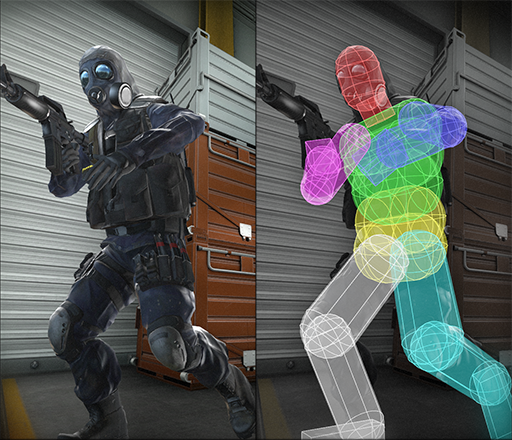
\includegraphics[width=1\textwidth]{./res/csgo_hitbox.png}
		\caption{Hitbox des Spieler-Modells aus dem Videospiel Counter Strike: Global Offensive; sichtbares Modell(links), mit eingeblendeter Hitbox (rechts)}
%%TODO source for pic
		\label{fig:chitbox}
	\end{subfigure}
~
	\begin{subfigure}[t]{0.2\textwidth}
		\centering
		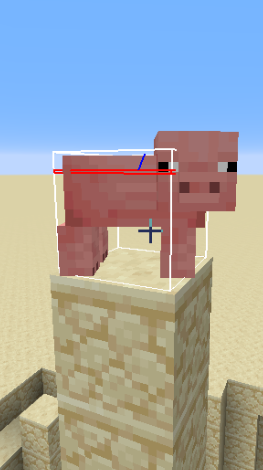
\includegraphics[width=1\textwidth]{./res/pig_hitbox.png}
		\caption{Hitbox eines NPC-Modells (Schwein) aus dem Videospiel Minecraft; Hitbox in weiß}
		\label{fig:mphitbox}
	\end{subfigure}
~
	\begin{subfigure}[t]{0.2\textwidth}
		\centering
		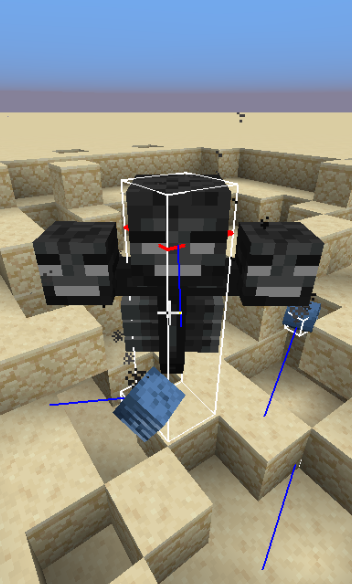
\includegraphics[width=1\textwidth]{./res/wither_hitbox.png}
		\caption{Hitbox eines NPC-Modells (Wither) aus dem Videospiel Minecraft; Hitbox in weiß}
		\label{fig:mwhitbox}
	\end{subfigure}

	\caption{Güten von Hitboxen}
	\label{fig:hitbox}
\end{figure*}

Die Abbildungen~\ref{fig:hitbox} zeigen Hitboxen in 2 verschiedenen Spielen.\\
\ref{fig:chitbox} zeigt das Spielermodell aus dem Spiel Counter-Strike: Global Offensive (CSGO). Links ist dabei das sichtbare Modell zu sehen, während rechts die Hitboxen eingeblendet sind. Die Hitboxen, welche hier nichmal mehr Boxen sind, sondern Ellipsoiden, decken das sichtbare Modell relativ genau ab. Ebenfalls zu erkennen ist die Partition in einzelne Hitboxen, zu sehen an den verschiedenen Farben der Hitboxen im rechten Bild.\\
Einzelne Details des Spielermodells, wie Riemen und Taschen an der Ausrüsung, sind nicht essentiell und werden daher auch physikalisch nicht abgebildet.\\
\ref{fig:mphitbox} und \ref{fig:mwhitbox} zeigen Hitboxen aus dem Spiel Minecraft bei zwei NPCs (Non-Player-Character (zu Deutsch: Nicht-Spieler-Charakter)). Es ist dort klar zu erkennen, dass die Hitboxen nicht sehr genau mit dem sichtbaren Modell übereinstimmen. Mehr noch: Die Minecraft-Hitboxen sind Koordinatenachsenparallel, d.h. Kanten verlaufen immer entlang der Koordinatenachsen der Raumrepräsentation.\\
Es wird versucht die Unterschiede zu rechtfertigen:\\
CSGO ist ein Shooter. Schnelle Reaktion und genaues Zielen sind ein hauptbestandteil des Produkts. Zudem ist CSGO ein hochkompetitiver E-Sport, der professionell gespielt wird. Es geht dabei um Preisgelder im siebenstelligen Bereich \cite{csgoprice}. Akkurate und, aus der perspektive des Spielers deterministische Hitboxen sind daher essenziell für das Produkt.\\
Die Partition der Hitboxen in CSGO ergibt sich direkt aus einer Anforderung der Anwendung, Schusstreffer auf verschiedene Teile des Spielermodells unterschiedlich zu bewerten. Beispielsweise verursacht der Treffer am Kopf am meisten Schaden. CSGO modelliert die unterschiedlichen Treffbaren teile des Modells also über mehrere Hitboxen.\\
Minecraft ist ein Sandbox Aufbauspiel. Ziel des Spiels ist der Bau von beliebigen Gebäuden, Tunneln, die Kreation von Maschinen oder das Erkunden von Gebieten.\\
In Minecraft steckt auch eine erhebliche Summe Geld. Am 15. September 2014 kaufte Microsoft die Entwicklerfirma und die rechte am Spiel für ca. 2,5 Milliarden Dollar \cite{buyminecraft}.\\
Das Kampfsystem in Minecraft forciert keine schnellen und genauen Treffer auf Gegner. Die gesamte Spielwelt ist aus sichtbaren Achsenparallel aufgestellten Würfeln gegeben, sind also Deckungsgleich mit entsprechenden achsenparallelen Hitboxen. Minecraft macht es sich einfach, da keine konkreten Anforderungen hinsichtlich Genauigkeit bestehen. Tatsächlich wird eine künstlich kleinere Hitbox manchmal sogar eingesetzt um einen Treffer zu erschweren (vgl. Abbildung \ref{fig::mwhitbox}).\\


\subsection{Hüllkörper}
Ein Bounding-Volume zu einem Objekt $o$ ist eine kompakte Menge $B_o \supset K_{o}$. $B_o$ kann als Hitbox fungieren.\\
Eine Bounding-Box ist ein spezielles Bounding-Volume in Form eines Quaders.\\
Eine in diesem Projekt extensiv verwendete, tiefere Spezialform der Bounding-Box ist die Axis-Alligned-Bounding-Box (AABB). Alle Kanten dieser Bounding-Box sind achsenparallel zu den Koordinatenachsen $\{(1,0,0), (0,1,0), (0,0,1)\}$ des 3D-Koordinatensystems.\\
Hier relevante Eigenschaften dieser sind:
\begin{itemize}
	\item kleine Datenrepresentation $AABB := (AABB_{o, min}, AABB) \in \mathcal{S}^{3^2}$ möglich.
		 In ihnen werden Minimal- und Maximalpositionen der AABB festgehalten.
	\item Schnelle Kollisionsüberprüfung zwischen AABBs durch Vergleiche der Extrema (Komplexität $= \mathcal{O}(1)$)
	\item Ermittlung einer minimalen AABB für ein Objekt durch Suche der Minima/Maxima (Komplexität $\le \mathcal{O}(n); n $ ist die Anzahl der Objektmerkmale (z.B. Ecken bei Polygon-Meshes))\\
		Die AABB muss sich an das eingeschlossene Objekt bei Bewegung anpassen. Standardmäßig durch Neuermittlung der AABB($\mathcal{O}(n)$). Optimierungen für verschiedene Arten von Bewegung möglich (Positionsänderung, Skalierung, etc.), aber manchmal schwierig (z.B. bei Rotation).
\end{itemize}

Im Falle des Spiels Minecraft werden AABBs als finale Hitboxen verwendet (vgl. \ref{fig:mwhitbox, fig:mphitbox}), welche jedoch scheinbar dem Kriterium $K_o \subseteq B_o$ zuwiderlaufen. Es muss an dieser Stelle zwischen der mathematischen Korrektheit einer Bounding-Box gegenüber einem gegebenen physikalischen Modell und der Designentscheidung gemacht werden, dass das sichtbare Modell nicht oder nur marginal die Grundlage des physikalischen Modells ist. In Minecraft ist die AABB die finale Hitbox  $H_{o, [min]} = K_o$ und definiert dadurch das Modell $K_o$. Das Bounding-Box-Kriterium ist damit theoretisch erfüllt. Die Designentscheidung selbst soll an dieser Stelle nicht eingeschätzt werden.



